% Options for packages loaded elsewhere
\PassOptionsToPackage{unicode}{hyperref}
\PassOptionsToPackage{hyphens}{url}
%
\documentclass[
]{article}
\usepackage{amsmath,amssymb}
\usepackage{lmodern}
\usepackage{iftex}
\ifPDFTeX
  \usepackage[T1]{fontenc}
  \usepackage[utf8]{inputenc}
  \usepackage{textcomp} % provide euro and other symbols
\else % if luatex or xetex
  \usepackage{unicode-math}
  \defaultfontfeatures{Scale=MatchLowercase}
  \defaultfontfeatures[\rmfamily]{Ligatures=TeX,Scale=1}
\fi
% Use upquote if available, for straight quotes in verbatim environments
\IfFileExists{upquote.sty}{\usepackage{upquote}}{}
\IfFileExists{microtype.sty}{% use microtype if available
  \usepackage[]{microtype}
  \UseMicrotypeSet[protrusion]{basicmath} % disable protrusion for tt fonts
}{}
\makeatletter
\@ifundefined{KOMAClassName}{% if non-KOMA class
  \IfFileExists{parskip.sty}{%
    \usepackage{parskip}
  }{% else
    \setlength{\parindent}{0pt}
    \setlength{\parskip}{6pt plus 2pt minus 1pt}}
}{% if KOMA class
  \KOMAoptions{parskip=half}}
\makeatother
\usepackage{xcolor}
\usepackage[margin=1in]{geometry}
\usepackage{color}
\usepackage{fancyvrb}
\newcommand{\VerbBar}{|}
\newcommand{\VERB}{\Verb[commandchars=\\\{\}]}
\DefineVerbatimEnvironment{Highlighting}{Verbatim}{commandchars=\\\{\}}
% Add ',fontsize=\small' for more characters per line
\usepackage{framed}
\definecolor{shadecolor}{RGB}{248,248,248}
\newenvironment{Shaded}{\begin{snugshade}}{\end{snugshade}}
\newcommand{\AlertTok}[1]{\textcolor[rgb]{0.94,0.16,0.16}{#1}}
\newcommand{\AnnotationTok}[1]{\textcolor[rgb]{0.56,0.35,0.01}{\textbf{\textit{#1}}}}
\newcommand{\AttributeTok}[1]{\textcolor[rgb]{0.77,0.63,0.00}{#1}}
\newcommand{\BaseNTok}[1]{\textcolor[rgb]{0.00,0.00,0.81}{#1}}
\newcommand{\BuiltInTok}[1]{#1}
\newcommand{\CharTok}[1]{\textcolor[rgb]{0.31,0.60,0.02}{#1}}
\newcommand{\CommentTok}[1]{\textcolor[rgb]{0.56,0.35,0.01}{\textit{#1}}}
\newcommand{\CommentVarTok}[1]{\textcolor[rgb]{0.56,0.35,0.01}{\textbf{\textit{#1}}}}
\newcommand{\ConstantTok}[1]{\textcolor[rgb]{0.00,0.00,0.00}{#1}}
\newcommand{\ControlFlowTok}[1]{\textcolor[rgb]{0.13,0.29,0.53}{\textbf{#1}}}
\newcommand{\DataTypeTok}[1]{\textcolor[rgb]{0.13,0.29,0.53}{#1}}
\newcommand{\DecValTok}[1]{\textcolor[rgb]{0.00,0.00,0.81}{#1}}
\newcommand{\DocumentationTok}[1]{\textcolor[rgb]{0.56,0.35,0.01}{\textbf{\textit{#1}}}}
\newcommand{\ErrorTok}[1]{\textcolor[rgb]{0.64,0.00,0.00}{\textbf{#1}}}
\newcommand{\ExtensionTok}[1]{#1}
\newcommand{\FloatTok}[1]{\textcolor[rgb]{0.00,0.00,0.81}{#1}}
\newcommand{\FunctionTok}[1]{\textcolor[rgb]{0.00,0.00,0.00}{#1}}
\newcommand{\ImportTok}[1]{#1}
\newcommand{\InformationTok}[1]{\textcolor[rgb]{0.56,0.35,0.01}{\textbf{\textit{#1}}}}
\newcommand{\KeywordTok}[1]{\textcolor[rgb]{0.13,0.29,0.53}{\textbf{#1}}}
\newcommand{\NormalTok}[1]{#1}
\newcommand{\OperatorTok}[1]{\textcolor[rgb]{0.81,0.36,0.00}{\textbf{#1}}}
\newcommand{\OtherTok}[1]{\textcolor[rgb]{0.56,0.35,0.01}{#1}}
\newcommand{\PreprocessorTok}[1]{\textcolor[rgb]{0.56,0.35,0.01}{\textit{#1}}}
\newcommand{\RegionMarkerTok}[1]{#1}
\newcommand{\SpecialCharTok}[1]{\textcolor[rgb]{0.00,0.00,0.00}{#1}}
\newcommand{\SpecialStringTok}[1]{\textcolor[rgb]{0.31,0.60,0.02}{#1}}
\newcommand{\StringTok}[1]{\textcolor[rgb]{0.31,0.60,0.02}{#1}}
\newcommand{\VariableTok}[1]{\textcolor[rgb]{0.00,0.00,0.00}{#1}}
\newcommand{\VerbatimStringTok}[1]{\textcolor[rgb]{0.31,0.60,0.02}{#1}}
\newcommand{\WarningTok}[1]{\textcolor[rgb]{0.56,0.35,0.01}{\textbf{\textit{#1}}}}
\usepackage{longtable,booktabs,array}
\usepackage{calc} % for calculating minipage widths
% Correct order of tables after \paragraph or \subparagraph
\usepackage{etoolbox}
\makeatletter
\patchcmd\longtable{\par}{\if@noskipsec\mbox{}\fi\par}{}{}
\makeatother
% Allow footnotes in longtable head/foot
\IfFileExists{footnotehyper.sty}{\usepackage{footnotehyper}}{\usepackage{footnote}}
\makesavenoteenv{longtable}
\usepackage{graphicx}
\makeatletter
\def\maxwidth{\ifdim\Gin@nat@width>\linewidth\linewidth\else\Gin@nat@width\fi}
\def\maxheight{\ifdim\Gin@nat@height>\textheight\textheight\else\Gin@nat@height\fi}
\makeatother
% Scale images if necessary, so that they will not overflow the page
% margins by default, and it is still possible to overwrite the defaults
% using explicit options in \includegraphics[width, height, ...]{}
\setkeys{Gin}{width=\maxwidth,height=\maxheight,keepaspectratio}
% Set default figure placement to htbp
\makeatletter
\def\fps@figure{htbp}
\makeatother
\setlength{\emergencystretch}{3em} % prevent overfull lines
\providecommand{\tightlist}{%
  \setlength{\itemsep}{0pt}\setlength{\parskip}{0pt}}
\setcounter{secnumdepth}{-\maxdimen} % remove section numbering
\ifLuaTeX
  \usepackage{selnolig}  % disable illegal ligatures
\fi
\IfFileExists{bookmark.sty}{\usepackage{bookmark}}{\usepackage{hyperref}}
\IfFileExists{xurl.sty}{\usepackage{xurl}}{} % add URL line breaks if available
\urlstyle{same} % disable monospaced font for URLs
\hypersetup{
  hidelinks,
  pdfcreator={LaTeX via pandoc}}

\title{UNIVERSIDADE FEDERAL DA BAHIA\\
INSTITUTO DE MATEMÁTICA E ESTATÍSTICA\\
\strut \\
\strut \\
\strut \\
FERNANDO\\
JEFF CAPONERO\\
\strut \\
\strut \\
\strut \\
\strut \\
\strut \\
\strut \\
Relatório de Atividade Laboratorial de Regressão}
\author{}
\date{\vspace{-2.5em}}

\begin{document}
\maketitle

{
\setcounter{tocdepth}{2}
\tableofcontents
}
\newpage

\hypertarget{apresentauxe7uxe3o}{%
\subsection{Apresentação}\label{apresentauxe7uxe3o}}

\newline
\newline

Este documento é um relatório referente a atividade de correlação e
dispersão de características associadas a relação da concentração de
glicose no plasma de mulheres da tribo Pina.

\hypertarget{introduuxe7uxe3o}{%
\subsection{Introdução}\label{introduuxe7uxe3o}}

\newline
\newline

O Instituto Nacional de Diabetes e de Doenças Digestivas e Renais dos
EUA conduziram um estudo com 768 mulheres da tribo Pina, que residem
próximo a Phoenix. As seguintes características foram coletadas: número
de gestações {[}pregnat{]}, concentração de glicose no plasma (obtido
duas horas depois da realização de um teste de tolerância a glicose)
{[}glucose{]}, pressão sanguínea diastólica (mmHg) {[}diastolic{]},
largura do tríceps (mm) {[}triceps{]}, nível de insulina (µU/ml)
{[}insulin{]}, índice de massa corpórea (kg/m2) {[}bmi{]}, nível de
função diabética {[}diabetes{]}, idade em anos {[}age{]} e um teste para
avaliação de sinais de diabetes (0 = negativo e 1 = positivo)
{[}teste{]}. Na base de dados as características estão rotuladas em
inglês conforme as indicações entre colchetes. Os resultados obitidos
foram avaliados e contrastados entre si.

\hypertarget{objetivos}{%
\subsection{Objetivos}\label{objetivos}}

\newline
\newline

\begin{enumerate}
\def\labelenumi{\arabic{enumi}.}
\tightlist
\item
  Sumarização dos dados do estudo.
\item
  Verificação de observações não usuais.
\item
  Relação da variável resposta (diabetes) com as demais variáveis.
\item
  Comparação do teste com as variáveis quantitativas e os níveis de
  glicose e de insulina, a pressão diastólica, o tríceps, o bmi, a idade
  e o nível de função diabética entre aqueles que apresentaram
  resultados do teste positivo e negativo.
\end{enumerate}

\newline
\newline

\hypertarget{sumarizauxe7uxe3o-dos-dados}{%
\subsection{Sumarização dos dados}\label{sumarizauxe7uxe3o-dos-dados}}

\newline
\newline

Com base nos dados disponíveis no arquivo ``Dados\_Lab01.csv'',
avaliou-se medidas de tendência central e de variabilidade além de se
construir um histograma para cada uma delas, como apresentado abaixo.

\newline

\textbf{Tabela 1 - Medidas de tendência central e de variabilidade dos
dados do estudo.}

\begin{longtable}[]{@{}lrrrrrr@{}}
\toprule()
& Mínimo & 1o Q. & Mediana & Média & 3o Q. & Máximo \\
\midrule()
\endhead
Gestações & 0.00 & 1.00 & 3.00 & 3.85 & 6.00 & 17.00 \\
Glicose & 0.00 & 99.00 & 117.00 & 120.89 & 140.25 & 199.00 \\
P. Diastólica & 0.00 & 62.00 & 72.00 & 69.11 & 80.00 & 122.00 \\
Tríceps & 0.00 & 0.00 & 23.00 & 20.54 & 32.00 & 99.00 \\
Insulina & 0.00 & 0.00 & 30.50 & 79.80 & 127.25 & 846.00 \\
IMC & 0.00 & 27.30 & 32.00 & 31.99 & 36.60 & 67.10 \\
N. Diabetes & 0.08 & 0.24 & 0.37 & 0.47 & 0.63 & 2.42 \\
Idade & 21.00 & 24.00 & 29.00 & 33.24 & 41.00 & 81.00 \\
\bottomrule()
\end{longtable}

\newpage

\textbf{Figura 1 - Resultado dos testes realizados nas mulheres da Tribo
Pina.}

\newline
\newline

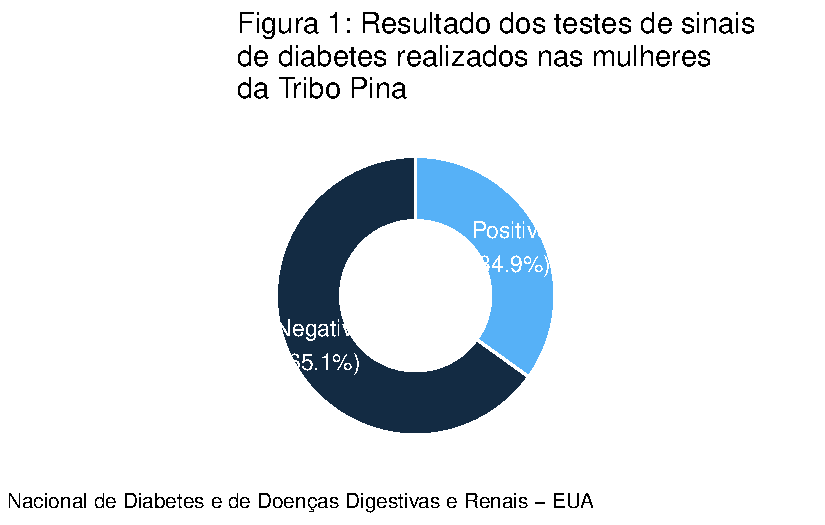
\includegraphics{Lab1---Jeff-Caponero_files/figure-latex/unnamed-chunk-3-1.pdf}
\newline \newline \newline

\textbf{Figura 2 - Histogramas dos dados do estudo.}

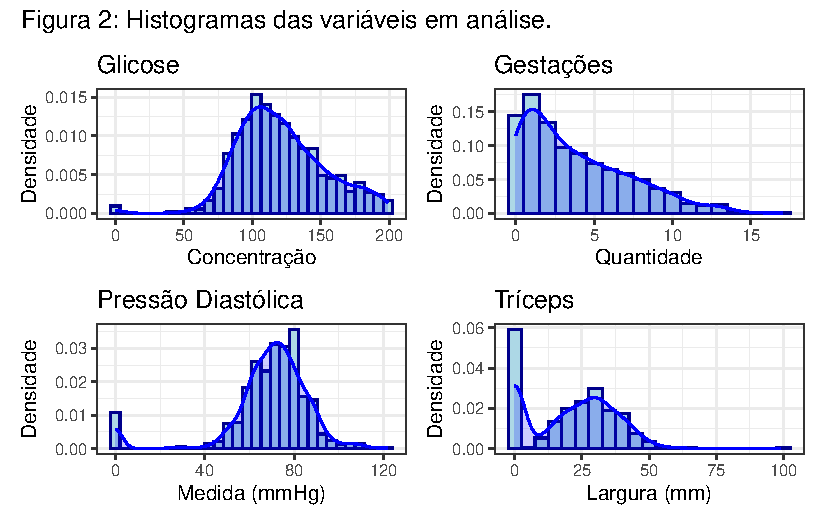
\includegraphics{Lab1---Jeff-Caponero_files/figure-latex/unnamed-chunk-4-1.pdf}
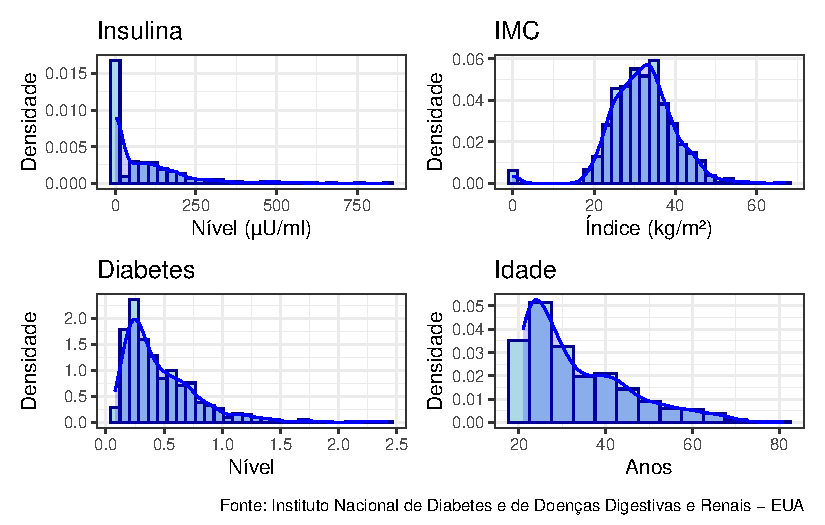
\includegraphics{Lab1---Jeff-Caponero_files/figure-latex/unnamed-chunk-4-2.pdf}

\newline
\newline
\newline
\newline

Observa-se que a presença de dados não usuais prejudicou a visualização
do comportamento de algumas variáveis, como é o caso do nível de glicose
no plasma, a pressão diastólica, a largura do tríceps, a concentração de
insulina e o índice de massa corpórea. Fazendo-se necessário um
tratamento dos dados analisados.

\newline
\newline

\hypertarget{tratamento-dos-dados}{%
\subsection{Tratamento dos dados}\label{tratamento-dos-dados}}

\newline
\newline

Observou-se a presença de dados cujo valor igual a zero não corresponde
a uma realidade plausível, desta forma, foram eliminados os registros
com esses valores e repetidos as análise anteriores.

\newline

\textbf{Tabela 2 - Medidas de tendência central e de variabilidade dos
dados do estudo sem observações não usuais.}

\begin{longtable}[]{@{}lrrrrrr@{}}
\toprule()
& Mínimo & 1o Q. & Mediana & Média & 3o Q. & Máximo \\
\midrule()
\endhead
Gestações & 0.00 & 1.00 & 2.00 & 3.30 & 5.00 & 17.00 \\
Glicose & 56.00 & 99.00 & 119.00 & 122.63 & 143.00 & 198.00 \\
P. Diastólica & 24.00 & 62.00 & 70.00 & 70.66 & 78.00 & 110.00 \\
Tríceps & 7.00 & 21.00 & 29.00 & 29.15 & 37.00 & 63.00 \\
Insulina & 14.00 & 76.75 & 125.50 & 156.06 & 190.00 & 846.00 \\
IMC & 18.20 & 28.40 & 33.20 & 33.09 & 37.10 & 67.10 \\
N. Diabetes & 0.09 & 0.27 & 0.45 & 0.52 & 0.69 & 2.42 \\
Idade & 21.00 & 23.00 & 27.00 & 30.86 & 36.00 & 81.00 \\
\bottomrule()
\end{longtable}

\newpage

\textbf{Figura 3 - Resultado dos testes realizados nas mulheres da Tribo
Pina.}

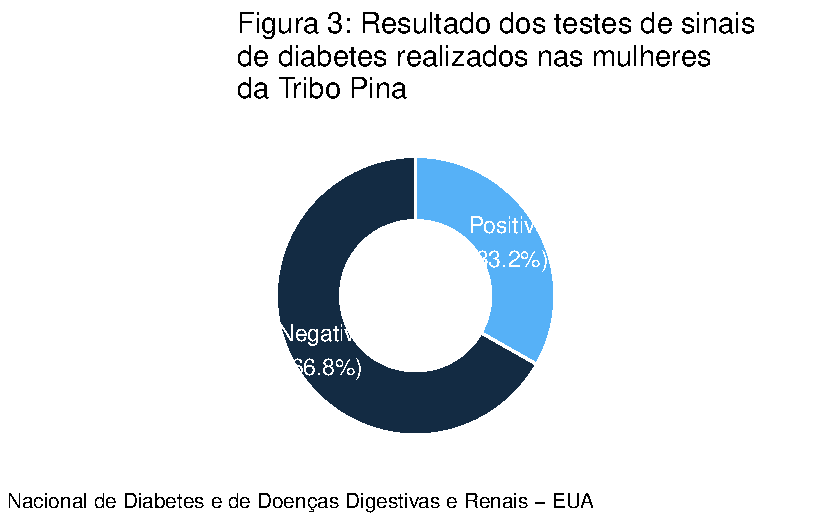
\includegraphics{Lab1---Jeff-Caponero_files/figure-latex/unnamed-chunk-6-1.pdf}

\newline

\textbf{Figura 4 - Histogramas dos dados do estudo sem observações não
usuais.}

\includegraphics{Lab1---Jeff-Caponero_files/figure-latex/unnamed-chunk-7-1.pdf}
\includegraphics{Lab1---Jeff-Caponero_files/figure-latex/unnamed-chunk-7-2.pdf}

\newline
\newline

Embora a eliminação dos registros com dados faltantes tenha melhorado a
a visualização do comportamento de algumas variáveis, como é o caso do
nível de glicose no plasma, a pressão diastólica, a largura do tríceps,
a concentração de insulina e o índice de massa corpórea; nota-se uma
perda de informação para as variáveis que estavam corretamente descritas
anteriormente como é o caso do número de gestações. Nota-se que o número
médio foi reduzido de 3,85 para 3,30. Semelhantemente, há perda de
informação para as variáveis nível de função diabética, idade e teste de
sinais de diabetes.

Observou-se ainda que algumas variáveis tem valores que parecem irreais,
como ó caso de largura de tríceps de 7mm ou nível de insulina de 849
µU/ml. Entretanto esta avaliação só pode ser feita por um especialista,
isto é, alguẽm capaz de definir intervalo valores possíveis para cada
variável.

\hypertarget{relauxe7uxe3o-da-variuxe1vel-diabetes-com-as-demais-variuxe1veis}{%
\subsection{Relação da variável diabetes com as demais
variáveis}\label{relauxe7uxe3o-da-variuxe1vel-diabetes-com-as-demais-variuxe1veis}}

\newpage

\textbf{Figura 5 - Diagramas de dispersão da relação da variável
resposta (diabetes) com as demais variáveis.}

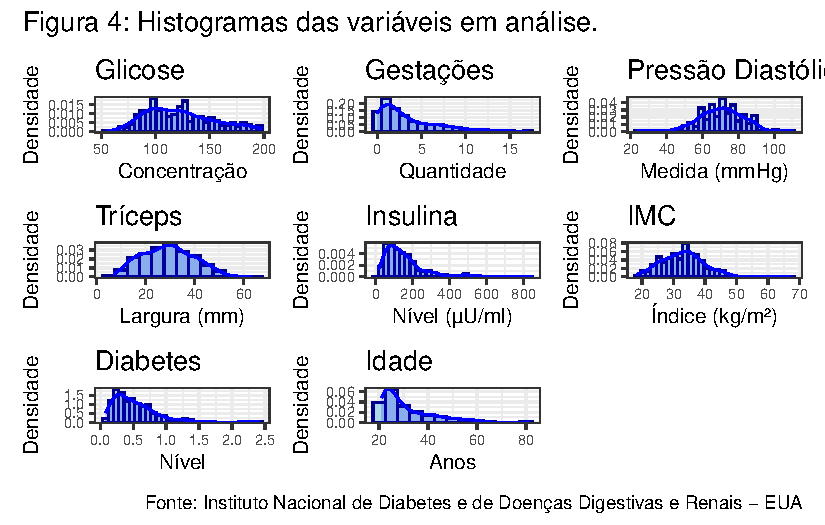
\includegraphics{Lab1---Jeff-Caponero_files/figure-latex/unnamed-chunk-8-1.pdf}
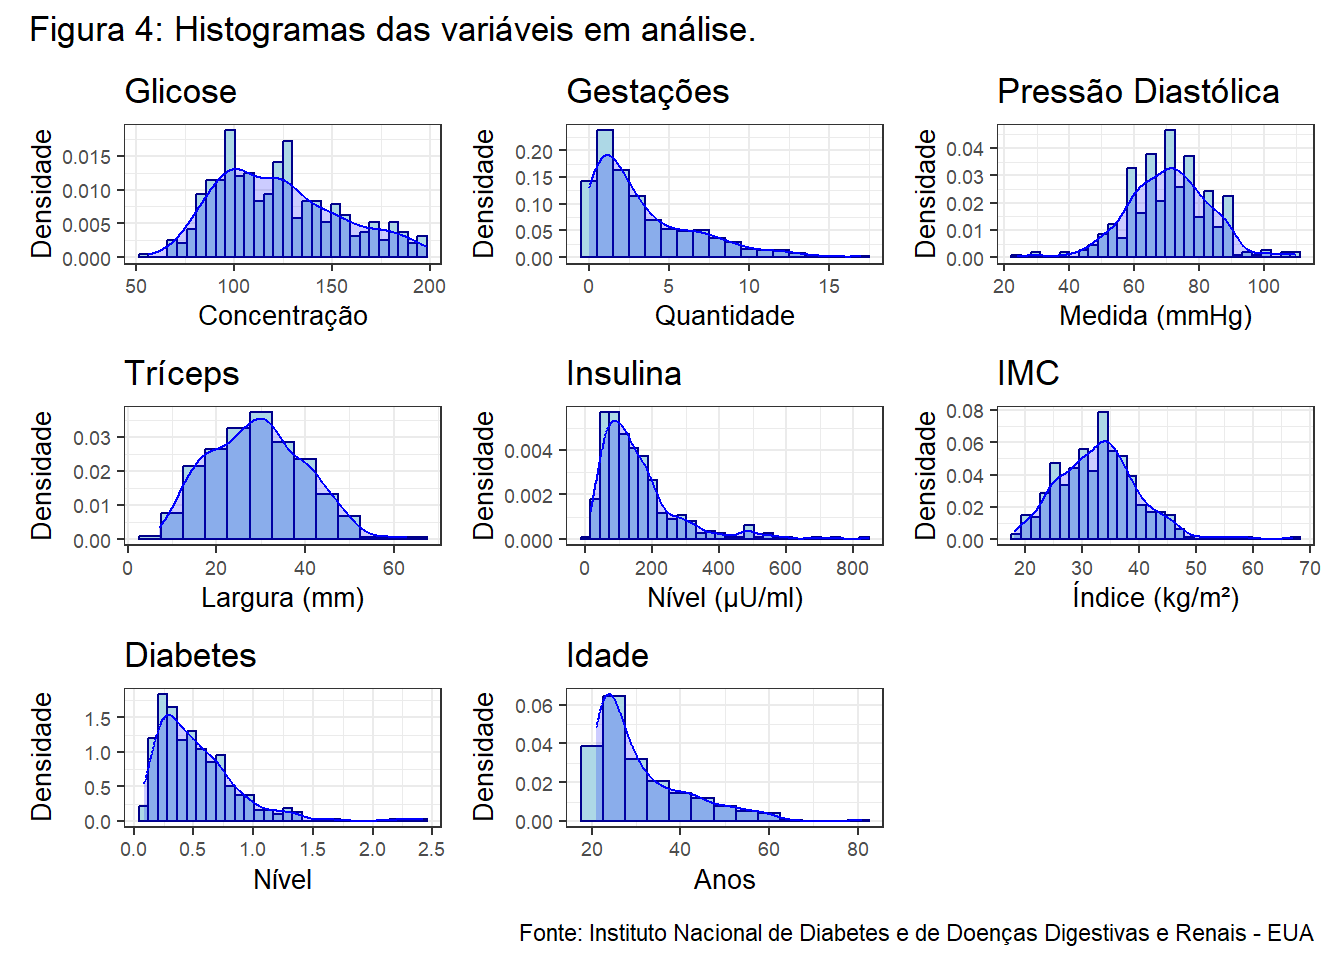
\includegraphics{Lab1---Jeff-Caponero_files/figure-latex/unnamed-chunk-8-2.pdf}

\newline
\newline

Visualmente nenhuma das características analizadas parece ter qualquer
correlação com o nível de função diabética.

\newpage

\textbf{Figura 6 - Boxplot do teste de sinais de diabetes com as demais
variáveis.}

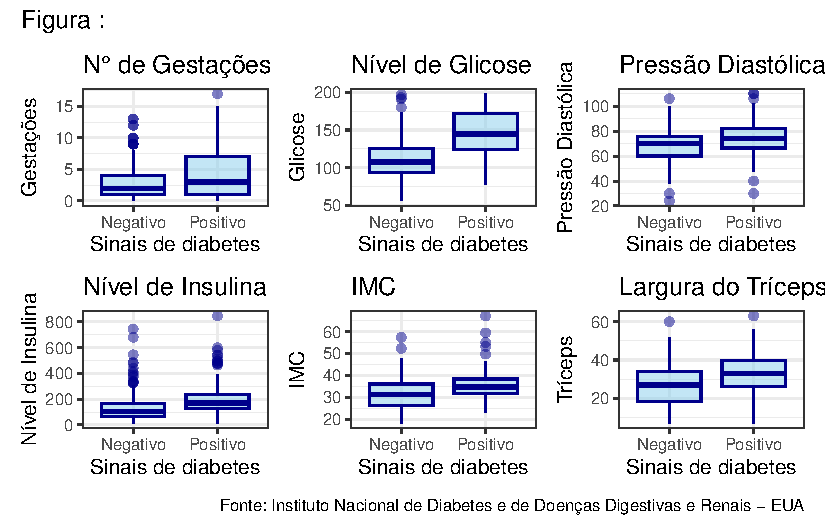
\includegraphics{Lab1---Jeff-Caponero_files/figure-latex/unnamed-chunk-9-1.pdf}
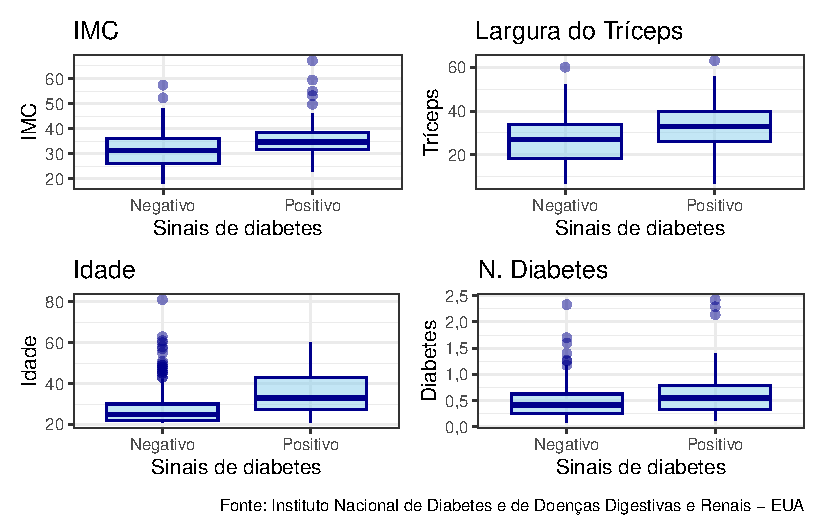
\includegraphics{Lab1---Jeff-Caponero_files/figure-latex/unnamed-chunk-9-2.pdf}

\newline
\newline

A análise dos bloxplots permite uma anális um pouco mais informativa,
uma vez que agora é possível verificar certa correlação entre o teste de
sinais de diabetes e as demais variáveis. Nota-se que esta correlação
não apresenta-se em grau superlativo, mas em níveis mais fracos.
Destacam-se os níveis de glicose no plasma e o nível de função diabética
com uma maior correlação, mas ainda assim sujeita a grande
variabilidade.

\hypertarget{conclusuxe3o}{%
\subsection{Conclusão}\label{conclusuxe3o}}

Com base nos resutadoa analisádos, velifica-se que não parece ser
suficiente a análise laboratorial na definição do estado de diabetes das
mulheres da Tribo Pina. Infere-se que a análise clinica pode se valer
das informações coletadas mas seu julgamento final deve contar com
outras técnicas disgnósticas.

\newpage

\hypertarget{apuxeandice}{%
\subsection{Apêndice}\label{apuxeandice}}

\hypertarget{cuxf3digo-em-linguagem-r}{%
\subsubsection{Código em linguagem R}\label{cuxf3digo-em-linguagem-r}}

\begin{Shaded}
\begin{Highlighting}[]
\DocumentationTok{\#\#\#\#\#\#\#\#\#\#\#\#\#\#\#\#\#\#\#\#\#\#\#\#\#\#\#\#\#\#\#\#\#\#\#\#\#\#\#\#\#\#\#\#\#\#}
\DocumentationTok{\#\#\#         Sumarização dos dados          }\AlertTok{\#\#\#}
\DocumentationTok{\#\#\#\#\#\#\#\#\#\#\#\#\#\#\#\#\#\#\#\#\#\#\#\#\#\#\#\#\#\#\#\#\#\#\#\#\#\#\#\#\#\#\#\#\#\#}
\FunctionTok{library}\NormalTok{(knitr)}
\FunctionTok{set.seed}\NormalTok{(}\DecValTok{7}\NormalTok{)}
\FunctionTok{setwd}\NormalTok{(}\StringTok{"\textasciitilde{}/Dropbox/Estatística/2023.1/Regressão/Exercícios"}\NormalTok{)}
\NormalTok{dados }\OtherTok{=} \FunctionTok{read.csv}\NormalTok{(}\StringTok{"Dados\_Lab01.csv"}\NormalTok{, }\AttributeTok{sep =} \StringTok{";"}\NormalTok{)}
\NormalTok{tab.gest }\OtherTok{=} \FunctionTok{summary}\NormalTok{(dados}\SpecialCharTok{$}\NormalTok{pregnant)}
\NormalTok{tab.gluc }\OtherTok{=} \FunctionTok{summary}\NormalTok{(dados}\SpecialCharTok{$}\NormalTok{glucose)}
\NormalTok{tab.dias }\OtherTok{=} \FunctionTok{summary}\NormalTok{(dados}\SpecialCharTok{$}\NormalTok{diastolic)}
\NormalTok{tab.tric }\OtherTok{=} \FunctionTok{summary}\NormalTok{(dados}\SpecialCharTok{$}\NormalTok{triceps)}
\NormalTok{tab.insu }\OtherTok{=} \FunctionTok{summary}\NormalTok{(dados}\SpecialCharTok{$}\NormalTok{insulin)}
\NormalTok{tab.bmi }\OtherTok{=} \FunctionTok{summary}\NormalTok{(dados}\SpecialCharTok{$}\NormalTok{bmi)}
\NormalTok{tab.diab }\OtherTok{=} \FunctionTok{summary}\NormalTok{(dados}\SpecialCharTok{$}\NormalTok{diabetes)}
\NormalTok{tab.age }\OtherTok{=} \FunctionTok{summary}\NormalTok{(dados}\SpecialCharTok{$}\NormalTok{age)}

\NormalTok{tab }\OtherTok{=} \FunctionTok{rbind}\NormalTok{(tab.gest,tab.gluc, tab.dias, tab.tric, tab.insu, tab.bmi, tab.diab, tab.age)}

\FunctionTok{colnames}\NormalTok{(tab) }\OtherTok{=} \FunctionTok{c}\NormalTok{(}\StringTok{"Mínimo"}\NormalTok{, }\StringTok{"1o Q."}\NormalTok{, }\StringTok{"Mediana"}\NormalTok{, }\StringTok{"Média"}\NormalTok{, }\StringTok{"3o Q."}\NormalTok{, }\StringTok{"Máximo"}\NormalTok{)}
\FunctionTok{rownames}\NormalTok{(tab) }\OtherTok{=} \FunctionTok{c}\NormalTok{(}\StringTok{"Gestações"}\NormalTok{, }\StringTok{"Glicose"}\NormalTok{, }\StringTok{"P. Diastólica"}\NormalTok{, }\StringTok{"Tríceps"}\NormalTok{, }\StringTok{"Insulina"}\NormalTok{, }\StringTok{"IMC"}\NormalTok{, }\StringTok{"N. Diabetes"}\NormalTok{, }\StringTok{"Idade"}\NormalTok{)}

\FunctionTok{kable}\NormalTok{(}\FunctionTok{round}\NormalTok{(tab,}\DecValTok{2}\NormalTok{))}

\CommentTok{\# Plot the chart.}
\NormalTok{tab.test }\OtherTok{=} \FunctionTok{table}\NormalTok{(dados}\SpecialCharTok{$}\NormalTok{test)}
\FunctionTok{rownames}\NormalTok{(tab.test) }\OtherTok{=} \FunctionTok{c}\NormalTok{(}\StringTok{"Negativo"}\NormalTok{, }\StringTok{"Positivo"}\NormalTok{)}
\FunctionTok{pie}\NormalTok{(tab.test)}

\FunctionTok{par}\NormalTok{(}\AttributeTok{mfrow =} \FunctionTok{c}\NormalTok{(}\DecValTok{2}\NormalTok{,}\DecValTok{2}\NormalTok{))}
\FunctionTok{hist}\NormalTok{(dados}\SpecialCharTok{$}\NormalTok{pregnant,}\AttributeTok{col=} \StringTok{"lightblue"}\NormalTok{, }\AttributeTok{breaks =} \DecValTok{10}\NormalTok{, }\AttributeTok{main =} \StringTok{"Gestações"}\NormalTok{, }\AttributeTok{xlab =} \StringTok{"Número de Gestações"}\NormalTok{)}
\FunctionTok{hist}\NormalTok{(dados}\SpecialCharTok{$}\NormalTok{glucose,}\AttributeTok{col=} \StringTok{"lightblue"}\NormalTok{, }\AttributeTok{breaks =} \DecValTok{10}\NormalTok{, }\AttributeTok{main =} \StringTok{"Glicose"}\NormalTok{, }\AttributeTok{xlab =} \StringTok{"Concentração no Plasma"}\NormalTok{)}

\FunctionTok{hist}\NormalTok{(dados}\SpecialCharTok{$}\NormalTok{diastolic,}\AttributeTok{col=} \StringTok{"lightblue"}\NormalTok{, }\AttributeTok{breaks =} \DecValTok{10}\NormalTok{, }\AttributeTok{main =} \StringTok{"Pressão Diastólica"}\NormalTok{, }\AttributeTok{xlab =} \StringTok{"Pressão Diastólica (mmHg)"}\NormalTok{)}
\FunctionTok{hist}\NormalTok{(dados}\SpecialCharTok{$}\NormalTok{triceps,}\AttributeTok{col=} \StringTok{"lightblue"}\NormalTok{, }\AttributeTok{breaks =} \DecValTok{10}\NormalTok{, }\AttributeTok{main =} \StringTok{"Largura do Tríceps"}\NormalTok{, }\AttributeTok{xlab =} \StringTok{"LArgura do Tríceps (mm)"}\NormalTok{)}

\FunctionTok{hist}\NormalTok{(dados}\SpecialCharTok{$}\NormalTok{insulin,}\AttributeTok{col=} \StringTok{"lightblue"}\NormalTok{, }\AttributeTok{breaks =} \DecValTok{10}\NormalTok{, }\AttributeTok{main =} \StringTok{"Insulina"}\NormalTok{, }\AttributeTok{xlab =} \StringTok{"Nível de Insulina (µU/ml)"}\NormalTok{)}
\FunctionTok{hist}\NormalTok{(dados}\SpecialCharTok{$}\NormalTok{bmi,}\AttributeTok{col=} \StringTok{"lightblue"}\NormalTok{, }\AttributeTok{breaks =} \DecValTok{10}\NormalTok{, }\AttributeTok{main =} \StringTok{"IMC"}\NormalTok{,}
     \AttributeTok{xlab =} \StringTok{"IMC (Kg/m2)"}\NormalTok{)}

\FunctionTok{hist}\NormalTok{(dados}\SpecialCharTok{$}\NormalTok{diabetes,}\AttributeTok{col=} \StringTok{"lightblue"}\NormalTok{, }\AttributeTok{breaks =} \DecValTok{10}\NormalTok{, }\AttributeTok{main =} \StringTok{"Diabetes"}\NormalTok{, }\AttributeTok{xlab =} \StringTok{"Nível de Função Diabética"}\NormalTok{)}
\FunctionTok{hist}\NormalTok{(dados}\SpecialCharTok{$}\NormalTok{age,}\AttributeTok{col=} \StringTok{"lightblue"}\NormalTok{, }\AttributeTok{breaks =} \DecValTok{10}\NormalTok{, }\AttributeTok{main =} \StringTok{"Idade"}\NormalTok{, }\AttributeTok{xlab =} \StringTok{"Idade (anos)"}\NormalTok{)}

\DocumentationTok{\#\#\#\#\#\#\#\#\#\#\#\#\#\#\#\#\#\#\#\#\#\#\#\#\#\#\#\#\#\#\#\#\#\#\#\#\#\#\#\#\#\#\#\#\#\#}
\DocumentationTok{\#\#\#          Tratamento dos dados          }\AlertTok{\#\#\#}
\DocumentationTok{\#\#\#\#\#\#\#\#\#\#\#\#\#\#\#\#\#\#\#\#\#\#\#\#\#\#\#\#\#\#\#\#\#\#\#\#\#\#\#\#\#\#\#\#\#\#}
\FunctionTok{library}\NormalTok{(dplyr)}
\NormalTok{dados }\OtherTok{=}\NormalTok{ dados }\SpecialCharTok{\%\textgreater{}\%} \FunctionTok{filter}\NormalTok{(glucose }\SpecialCharTok{!=} \DecValTok{0}\NormalTok{)}
\NormalTok{dados }\OtherTok{=}\NormalTok{ dados }\SpecialCharTok{\%\textgreater{}\%} \FunctionTok{filter}\NormalTok{(diastolic }\SpecialCharTok{!=} \DecValTok{0}\NormalTok{)}
\NormalTok{dados }\OtherTok{=}\NormalTok{ dados }\SpecialCharTok{\%\textgreater{}\%} \FunctionTok{filter}\NormalTok{(triceps }\SpecialCharTok{!=} \DecValTok{0}\NormalTok{)}
\NormalTok{dados }\OtherTok{=}\NormalTok{ dados }\SpecialCharTok{\%\textgreater{}\%} \FunctionTok{filter}\NormalTok{(insulin }\SpecialCharTok{!=} \DecValTok{0}\NormalTok{)}
\NormalTok{dados }\OtherTok{=}\NormalTok{ dados }\SpecialCharTok{\%\textgreater{}\%} \FunctionTok{filter}\NormalTok{(bmi }\SpecialCharTok{!=} \DecValTok{0}\NormalTok{)}
\NormalTok{dados }\OtherTok{=}\NormalTok{ dados }\SpecialCharTok{\%\textgreater{}\%} \FunctionTok{filter}\NormalTok{(diabetes }\SpecialCharTok{!=} \DecValTok{0}\NormalTok{)}
\NormalTok{dados }\OtherTok{=}\NormalTok{ dados }\SpecialCharTok{\%\textgreater{}\%} \FunctionTok{filter}\NormalTok{(age }\SpecialCharTok{!=} \DecValTok{0}\NormalTok{)}


\NormalTok{tab.gest }\OtherTok{=} \FunctionTok{summary}\NormalTok{(dados}\SpecialCharTok{$}\NormalTok{pregnant)}
\NormalTok{tab.gluc }\OtherTok{=} \FunctionTok{summary}\NormalTok{(dados}\SpecialCharTok{$}\NormalTok{glucose)}
\NormalTok{tab.dias }\OtherTok{=} \FunctionTok{summary}\NormalTok{(dados}\SpecialCharTok{$}\NormalTok{diastolic)}
\NormalTok{tab.tric }\OtherTok{=} \FunctionTok{summary}\NormalTok{(dados}\SpecialCharTok{$}\NormalTok{triceps)}
\NormalTok{tab.insu }\OtherTok{=} \FunctionTok{summary}\NormalTok{(dados}\SpecialCharTok{$}\NormalTok{insulin)}
\NormalTok{tab.bmi }\OtherTok{=} \FunctionTok{summary}\NormalTok{(dados}\SpecialCharTok{$}\NormalTok{bmi)}
\NormalTok{tab.diab }\OtherTok{=} \FunctionTok{summary}\NormalTok{(dados}\SpecialCharTok{$}\NormalTok{diabetes)}
\NormalTok{tab.age }\OtherTok{=} \FunctionTok{summary}\NormalTok{(dados}\SpecialCharTok{$}\NormalTok{age)}

\NormalTok{tab }\OtherTok{=} \FunctionTok{rbind}\NormalTok{(tab.gest,tab.gluc, tab.dias, tab.tric, tab.insu, tab.bmi, tab.diab, tab.age)}

\FunctionTok{colnames}\NormalTok{(tab) }\OtherTok{=} \FunctionTok{c}\NormalTok{(}\StringTok{"Mínimo"}\NormalTok{, }\StringTok{"1o Q."}\NormalTok{, }\StringTok{"Mediana"}\NormalTok{, }\StringTok{"Média"}\NormalTok{, }\StringTok{"3o Q."}\NormalTok{, }\StringTok{"Máximo"}\NormalTok{)}
\FunctionTok{rownames}\NormalTok{(tab) }\OtherTok{=} \FunctionTok{c}\NormalTok{(}\StringTok{"Gestações"}\NormalTok{, }\StringTok{"Glicose"}\NormalTok{, }\StringTok{"P. Diastólica"}\NormalTok{, }\StringTok{"Tríceps"}\NormalTok{, }\StringTok{"Insulina"}\NormalTok{, }\StringTok{"IMC"}\NormalTok{, }\StringTok{"N. Diabetes"}\NormalTok{, }\StringTok{"Idade"}\NormalTok{)}

\FunctionTok{kable}\NormalTok{(}\FunctionTok{round}\NormalTok{(tab,}\DecValTok{2}\NormalTok{))}

\CommentTok{\# Plot the chart.}
\NormalTok{tab.test }\OtherTok{=} \FunctionTok{table}\NormalTok{(dados}\SpecialCharTok{$}\NormalTok{test)}
\FunctionTok{rownames}\NormalTok{(tab.test) }\OtherTok{=} \FunctionTok{c}\NormalTok{(}\StringTok{"Negativo"}\NormalTok{, }\StringTok{"Positivo"}\NormalTok{)}
\FunctionTok{pie}\NormalTok{(tab.test)}

\FunctionTok{par}\NormalTok{(}\AttributeTok{mfrow =} \FunctionTok{c}\NormalTok{(}\DecValTok{2}\NormalTok{,}\DecValTok{2}\NormalTok{))}
\FunctionTok{hist}\NormalTok{(dados}\SpecialCharTok{$}\NormalTok{pregnant,}\AttributeTok{col=} \StringTok{"lightblue"}\NormalTok{, }\AttributeTok{breaks =} \DecValTok{10}\NormalTok{, }\AttributeTok{main =} \StringTok{"Gestações"}\NormalTok{, }\AttributeTok{xlab =} \StringTok{"Número de Gestações"}\NormalTok{)}
\FunctionTok{hist}\NormalTok{(dados}\SpecialCharTok{$}\NormalTok{glucose,}\AttributeTok{col=} \StringTok{"lightblue"}\NormalTok{, }\AttributeTok{breaks =} \DecValTok{10}\NormalTok{, }\AttributeTok{main =} \StringTok{"Glicose"}\NormalTok{, }\AttributeTok{xlab =} \StringTok{"Concentração no Plasma"}\NormalTok{)}

\FunctionTok{hist}\NormalTok{(dados}\SpecialCharTok{$}\NormalTok{diastolic,}\AttributeTok{col=} \StringTok{"lightblue"}\NormalTok{, }\AttributeTok{breaks =} \DecValTok{10}\NormalTok{, }\AttributeTok{main =} \StringTok{"Pressão Diastólica"}\NormalTok{, }\AttributeTok{xlab =} \StringTok{"Pressão Diastólica (mmHg)"}\NormalTok{)}
\FunctionTok{hist}\NormalTok{(dados}\SpecialCharTok{$}\NormalTok{triceps,}\AttributeTok{col=} \StringTok{"lightblue"}\NormalTok{, }\AttributeTok{breaks =} \DecValTok{10}\NormalTok{, }\AttributeTok{main =} \StringTok{"Largura do Tríceps"}\NormalTok{, }\AttributeTok{xlab =} \StringTok{"LArgura do Tríceps (mm)"}\NormalTok{)}

\FunctionTok{hist}\NormalTok{(dados}\SpecialCharTok{$}\NormalTok{insulin,}\AttributeTok{col=} \StringTok{"lightblue"}\NormalTok{, }\AttributeTok{breaks =} \DecValTok{10}\NormalTok{, }\AttributeTok{main =} \StringTok{"Insulina"}\NormalTok{, }\AttributeTok{xlab =} \StringTok{"Nível de Insulina (µU/ml)"}\NormalTok{)}
\FunctionTok{hist}\NormalTok{(dados}\SpecialCharTok{$}\NormalTok{bmi,}\AttributeTok{col=} \StringTok{"lightblue"}\NormalTok{, }\AttributeTok{breaks =} \DecValTok{10}\NormalTok{, }\AttributeTok{main =} \StringTok{"IMC"}\NormalTok{,}
     \AttributeTok{xlab =} \StringTok{"IMC (Kg/m2)"}\NormalTok{)}

\FunctionTok{hist}\NormalTok{(dados}\SpecialCharTok{$}\NormalTok{diabetes,}\AttributeTok{col=} \StringTok{"lightblue"}\NormalTok{, }\AttributeTok{breaks =} \DecValTok{10}\NormalTok{, }\AttributeTok{main =} \StringTok{"Diabetes"}\NormalTok{, }\AttributeTok{xlab =} \StringTok{"Nível de Função Diabética"}\NormalTok{)}
\FunctionTok{hist}\NormalTok{(dados}\SpecialCharTok{$}\NormalTok{age,}\AttributeTok{col=} \StringTok{"lightblue"}\NormalTok{, }\AttributeTok{breaks =} \DecValTok{10}\NormalTok{, }\AttributeTok{main =} \StringTok{"Idade"}\NormalTok{, }\AttributeTok{xlab =} \StringTok{"Idade (anos)"}\NormalTok{)}



\DocumentationTok{\#\#\#\#\#\#\#\#\#\#\#\#\#\#\#\#\#\#\#\#\#\#\#\#\#\#\#\#\#\#\#\#\#\#\#\#\#\#\#\#\#\#\#\#\#\#}
\DocumentationTok{\#\#\#          Diagramas de Dispersão        }\AlertTok{\#\#\#}
\DocumentationTok{\#\#\#\#\#\#\#\#\#\#\#\#\#\#\#\#\#\#\#\#\#\#\#\#\#\#\#\#\#\#\#\#\#\#\#\#\#\#\#\#\#\#\#\#\#\#}

\FunctionTok{par}\NormalTok{(}\AttributeTok{mfrow =} \FunctionTok{c}\NormalTok{(}\DecValTok{2}\NormalTok{,}\DecValTok{2}\NormalTok{))}
\FunctionTok{plot}\NormalTok{(dados}\SpecialCharTok{$}\NormalTok{pregnant, dados}\SpecialCharTok{$}\NormalTok{diabetes,   }\AttributeTok{col=} \StringTok{"lightblue"}\NormalTok{, }\AttributeTok{main =} \StringTok{"Gestações"}\NormalTok{, }\AttributeTok{xlab =} \StringTok{"Número de Gestações"}\NormalTok{, }\AttributeTok{ylab =} \StringTok{"Nível de Função Diabética"}\NormalTok{)}
\FunctionTok{plot}\NormalTok{(dados}\SpecialCharTok{$}\NormalTok{glucose, dados}\SpecialCharTok{$}\NormalTok{diabetes, }\AttributeTok{col=} \StringTok{"lightblue"}\NormalTok{, }\AttributeTok{main =} \StringTok{"Glicose"}\NormalTok{, }\AttributeTok{xlab =} \StringTok{"Concentração no Plasma"}\NormalTok{, }\AttributeTok{ylab =} \StringTok{"Nível de Função Diabética"}\NormalTok{)}

\FunctionTok{plot}\NormalTok{(dados}\SpecialCharTok{$}\NormalTok{diastolic, dados}\SpecialCharTok{$}\NormalTok{diabetes, }\AttributeTok{col=} \StringTok{"lightblue"}\NormalTok{, }\AttributeTok{main =} \StringTok{"Pressão Diastólica"}\NormalTok{, }\AttributeTok{xlab =} \StringTok{"Pressão Diastólica (mmHg)"}\NormalTok{, }\AttributeTok{ylab =} \StringTok{"Nível de Função Diabética"}\NormalTok{)}
\FunctionTok{plot}\NormalTok{(dados}\SpecialCharTok{$}\NormalTok{triceps, dados}\SpecialCharTok{$}\NormalTok{diabetes, }\AttributeTok{col=} \StringTok{"lightblue"}\NormalTok{, }\AttributeTok{main =} \StringTok{"Largura do Tríceps"}\NormalTok{, }\AttributeTok{xlab =} \StringTok{"Largura do Tríceps (mm)"}\NormalTok{, }\AttributeTok{ylab =} \StringTok{"Nível de Função Diabética"}\NormalTok{)}

\FunctionTok{plot}\NormalTok{(dados}\SpecialCharTok{$}\NormalTok{insulin, dados}\SpecialCharTok{$}\NormalTok{diabetes, }\AttributeTok{col=} \StringTok{"lightblue"}\NormalTok{, }\AttributeTok{main =} \StringTok{"Insulina"}\NormalTok{, }\AttributeTok{xlab =} \StringTok{"Nível de Insulina (µU/ml)"}\NormalTok{, }\AttributeTok{ylab =} \StringTok{"Nível de Função Diabética"}\NormalTok{)}
\FunctionTok{plot}\NormalTok{(dados}\SpecialCharTok{$}\NormalTok{bmi, dados}\SpecialCharTok{$}\NormalTok{diabetes, }\AttributeTok{col=} \StringTok{"lightblue"}\NormalTok{, }\AttributeTok{main =} \StringTok{"IMC"}\NormalTok{,}
     \AttributeTok{xlab =} \StringTok{"IMC (Kg/m2)"}\NormalTok{, }\AttributeTok{ylab =} \StringTok{"Nível de Função Diabética"}\NormalTok{)}

\FunctionTok{plot}\NormalTok{(dados}\SpecialCharTok{$}\NormalTok{age, dados}\SpecialCharTok{$}\NormalTok{diabetes, }\AttributeTok{col=} \StringTok{"lightblue"}\NormalTok{, }\AttributeTok{main =} \StringTok{"Idade"}\NormalTok{, }\AttributeTok{xlab =} \StringTok{"Idade (anos)"}\NormalTok{, }\AttributeTok{ylab =} \StringTok{"Nível de Função Diabética"}\NormalTok{)}

\DocumentationTok{\#\#\#\#\#\#\#\#\#\#\#\#\#\#\#\#\#\#\#\#\#\#\#\#\#\#\#\#\#\#\#\#\#\#\#\#\#\#\#\#\#\#\#\#\#\#}
\DocumentationTok{\#\#\#          Boxplot  dos Testes           }\AlertTok{\#\#\#}
\DocumentationTok{\#\#\#\#\#\#\#\#\#\#\#\#\#\#\#\#\#\#\#\#\#\#\#\#\#\#\#\#\#\#\#\#\#\#\#\#\#\#\#\#\#\#\#\#\#\#}

\FunctionTok{par}\NormalTok{(}\AttributeTok{mfrow =} \FunctionTok{c}\NormalTok{(}\DecValTok{2}\NormalTok{,}\DecValTok{2}\NormalTok{))}
\FunctionTok{boxplot}\NormalTok{(dados}\SpecialCharTok{$}\NormalTok{pregnant }\SpecialCharTok{\textasciitilde{}}\NormalTok{ dados}\SpecialCharTok{$}\NormalTok{test, }\AttributeTok{col=} \StringTok{"lightblue"}\NormalTok{, }\AttributeTok{main =} \StringTok{"Gestações"}\NormalTok{, }\AttributeTok{ylab =} \StringTok{"Número de Gestações"}\NormalTok{, }\AttributeTok{xlab =} \StringTok{"Teste de Sinais de Diabetes"}\NormalTok{)}
\FunctionTok{boxplot}\NormalTok{(dados}\SpecialCharTok{$}\NormalTok{glucose }\SpecialCharTok{\textasciitilde{}}\NormalTok{ dados}\SpecialCharTok{$}\NormalTok{test, }\AttributeTok{col=} \StringTok{"lightblue"}\NormalTok{, }\AttributeTok{main =} \StringTok{"Gestações"}\NormalTok{, }\AttributeTok{ylab =} \StringTok{"Concentração no Plasma"}\NormalTok{, }\AttributeTok{xlab =} \StringTok{"Teste de Sinais de Diabetes"}\NormalTok{)}

\FunctionTok{boxplot}\NormalTok{(dados}\SpecialCharTok{$}\NormalTok{diastolic }\SpecialCharTok{\textasciitilde{}}\NormalTok{ dados}\SpecialCharTok{$}\NormalTok{test, }\AttributeTok{col=} \StringTok{"lightblue"}\NormalTok{, }\AttributeTok{main =} \StringTok{"Gestações"}\NormalTok{, }\AttributeTok{ylab =} \StringTok{"Pressão Diastólica (mmHg)"}\NormalTok{, }\AttributeTok{xlab =} \StringTok{"Teste de Sinais de Diabetes"}\NormalTok{)}
\FunctionTok{boxplot}\NormalTok{(dados}\SpecialCharTok{$}\NormalTok{triceps }\SpecialCharTok{\textasciitilde{}}\NormalTok{ dados}\SpecialCharTok{$}\NormalTok{test,}\AttributeTok{col=} \StringTok{"lightblue"}\NormalTok{, }\AttributeTok{main =} \StringTok{"Gestações"}\NormalTok{, }\AttributeTok{ylab =} \StringTok{"Largura do Tríceps (mm)"}\NormalTok{, }\AttributeTok{xlab =} \StringTok{"Teste de Sinais de Diabetes"}\NormalTok{)}

\FunctionTok{boxplot}\NormalTok{(dados}\SpecialCharTok{$}\NormalTok{insulin }\SpecialCharTok{\textasciitilde{}}\NormalTok{ dados}\SpecialCharTok{$}\NormalTok{test,}\AttributeTok{col=} \StringTok{"lightblue"}\NormalTok{, }\AttributeTok{main =} \StringTok{"Gestações"}\NormalTok{, }\AttributeTok{ylab =} \StringTok{"Nível de Insulina (µU/ml)"}\NormalTok{, }\AttributeTok{xlab =} \StringTok{"Teste de Sinais de Diabetes"}\NormalTok{)}
\FunctionTok{boxplot}\NormalTok{(dados}\SpecialCharTok{$}\NormalTok{bmi }\SpecialCharTok{\textasciitilde{}}\NormalTok{ dados}\SpecialCharTok{$}\NormalTok{test,}\AttributeTok{col=} \StringTok{"lightblue"}\NormalTok{, }\AttributeTok{main =} \StringTok{"Gestações"}\NormalTok{, }\AttributeTok{ylab =} \StringTok{"IMC (Kg/m2)"}\NormalTok{, }\AttributeTok{xlab =} \StringTok{"Teste de Sinais de Diabetes"}\NormalTok{)}

\FunctionTok{boxplot}\NormalTok{(dados}\SpecialCharTok{$}\NormalTok{diabetes }\SpecialCharTok{\textasciitilde{}}\NormalTok{ dados}\SpecialCharTok{$}\NormalTok{test,}\AttributeTok{col=} \StringTok{"lightblue"}\NormalTok{, }\AttributeTok{main =} \StringTok{"Gestações"}\NormalTok{, }\AttributeTok{ylab =} \StringTok{"Nível de Função Diabética"}\NormalTok{, }\AttributeTok{xlab =} \StringTok{"Teste de Sinais de Diabetes"}\NormalTok{)}
\FunctionTok{boxplot}\NormalTok{(dados}\SpecialCharTok{$}\NormalTok{age }\SpecialCharTok{\textasciitilde{}}\NormalTok{ dados}\SpecialCharTok{$}\NormalTok{test,}\AttributeTok{col=} \StringTok{"lightblue"}\NormalTok{, }\AttributeTok{main =} \StringTok{"Gestações"}\NormalTok{, }\AttributeTok{ylab =} \StringTok{"Idade (anos)"}\NormalTok{, }\AttributeTok{xlab =} \StringTok{"Teste de Sinais de Diabetes"}\NormalTok{)}
\end{Highlighting}
\end{Shaded}


\end{document}
